\documentclass[a4paper, 12pt]{article}
\usepackage{barinov}
\begin{document}
\thispagestyle{empty}
\begin{center}
    \textit{Федеральное государственное автономное образовательное\\ учреждение высшего образования }

    \vspace{0.5ex}

        \textbf{«Московский физико-технический институт\\ (национальный исследовательский университет)»}
\end{center}

\vspace{10ex}

\begin{center}
    \vspace{13ex}

    \so{\textbf{Лабораторная работа №_._._}}

    \vspace{1ex}

    по курсу общей физики

    на тему:

    \textbf{\textit{<<>>}}

    \vspace{30ex}

    \begin{flushright}
        \noindent
        \textit{Работу выполнил:}\\  
        \textit{Баринов Леонид \\(группа Б02-827)}
    \end{flushright}
    \vfill
    Долгопрудный \\2019
\newpage
\setcounter{page}{1}
\fancyhead[R]{\nouppercase{\leftmark}}	
\end{center}

\section{Аннотация}
В работе будет исследована интерференция рассеянного света, прошедшего
кристалл. Проведено наблюдение изменения характера поляризации света
при наложении на кристалл электрического поля.






\section{Теоретические сведения}
Эффектом Поккельса называется изменение показателя преломления света в
кристалле под действием электрического поля, причем это изменение
пропорционально напряженности электрического поля. Вследствие эффекта
Поккельса в кристалле либо появляется двойное лучепреломление, либо
меняется его величина, либо, как в данной работе, одноосный кристалл
становится двуосным.

Рассмотрим сначала кристалл в отсутствие внешнего электрического поля.
Кристалл ниобата лития является одноосным кристаллом, то есть
кристаллом, оптические свойства которого обладают симметрией вращения
относительно некоторого одного направления, называемого оптической
осью $z$ кристалла. Для световой волны, вектор электрического поля
$\vv{E}$ которой перпендикулярен оси $z$, показатель преломления равен
$n_o = \sqrt{\epsilon_\perp}$, а для волны, вектор $\vv{E}$ которой
располагается вдоль оси $z$, он равен $n_e = \sqrt{\epsilon_\|}$,
причем $n_e<n_o$, т.е. LiNbO$_3$ - <<отрицательный кристалл>>.


\begin{figure}[H]
    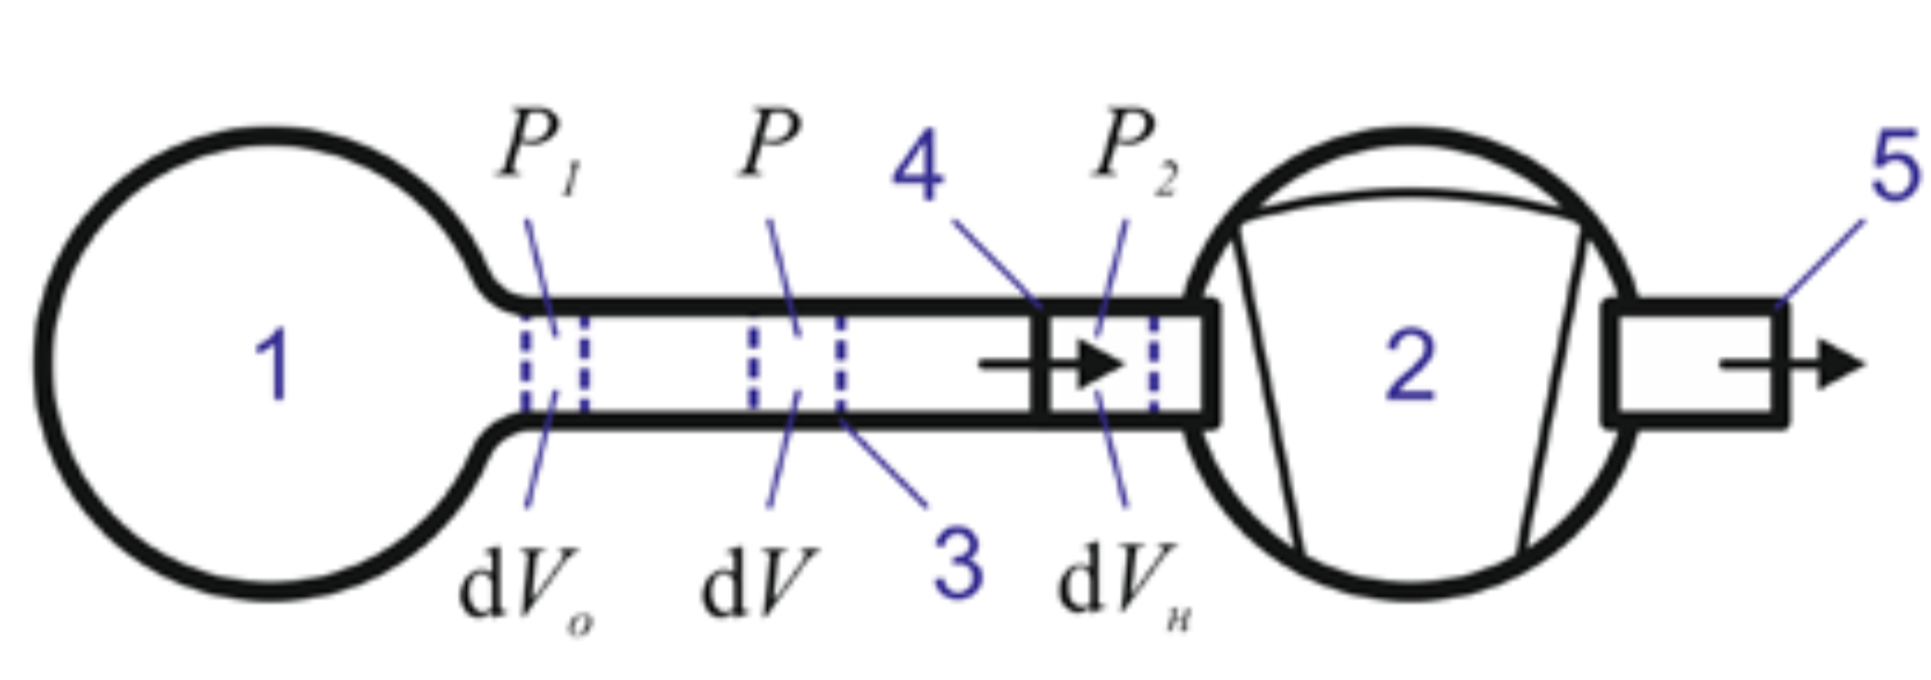
\includegraphics[width=0.8\linewidth]{1} 
    \caption{Схема для наблюдения интерференционной картины}
    \label{fig:1}
\end{figure}

В общем случае, когда луч света распространяется под углом $\theta$ к
оптической оси $z$ (\fig{fig:1}), существует два собственных значения
показателя преломления $n_1$ и $n_2$: в обыкновенной волне (если
световой вектор $\vv{E}$ перпендикулярен плоскости
$(\vv{k},\vv{e}_z)$, где $\vv{k}$ --- волновой вектор луча, $\vv{e}_z$
--- орт по оси $z$) показатель $n_1 = n_o$, а в необыкновенной (когда
световой вектор $\vv{E}$ лежит в плоскости $(\vv{k},\vv{e}_z)$)
показатель преломления $n_2$ зависит от угла $\theta$:
\begin{equation}
    \frac{1}{n_2^2} = \frac{\cos^2 \theta}{n_o^2} + \frac{\sin^2
    \theta}{n_e^2}
    \label{eq:1}
\end{equation}

Для $m$-го темного кольца $\Delta \phi = 2\pi m$ или $\Delta \phi =
2\pi/\lambda \cdot l (n_o-n_e)\theta^2 = 2\pi m$. Если $L$ ---
расстояние от центра кристалла до экрана, то, учитывая закон
преломления на границе кристалла, при малых углах $\theta_\text{внешн}
= n_o \theta$ (\fig{fig:1}) получаем выражение для радиуса кольца:
\begin{equation}
    r_m^2 = \frac{\lambda}{l} \frac{(n_o L)^2}{(n_o-n_e)} m
    \label{eq:2}
\end{equation}

\begin{wrapfigure}{r}{0.4\linewidth}
    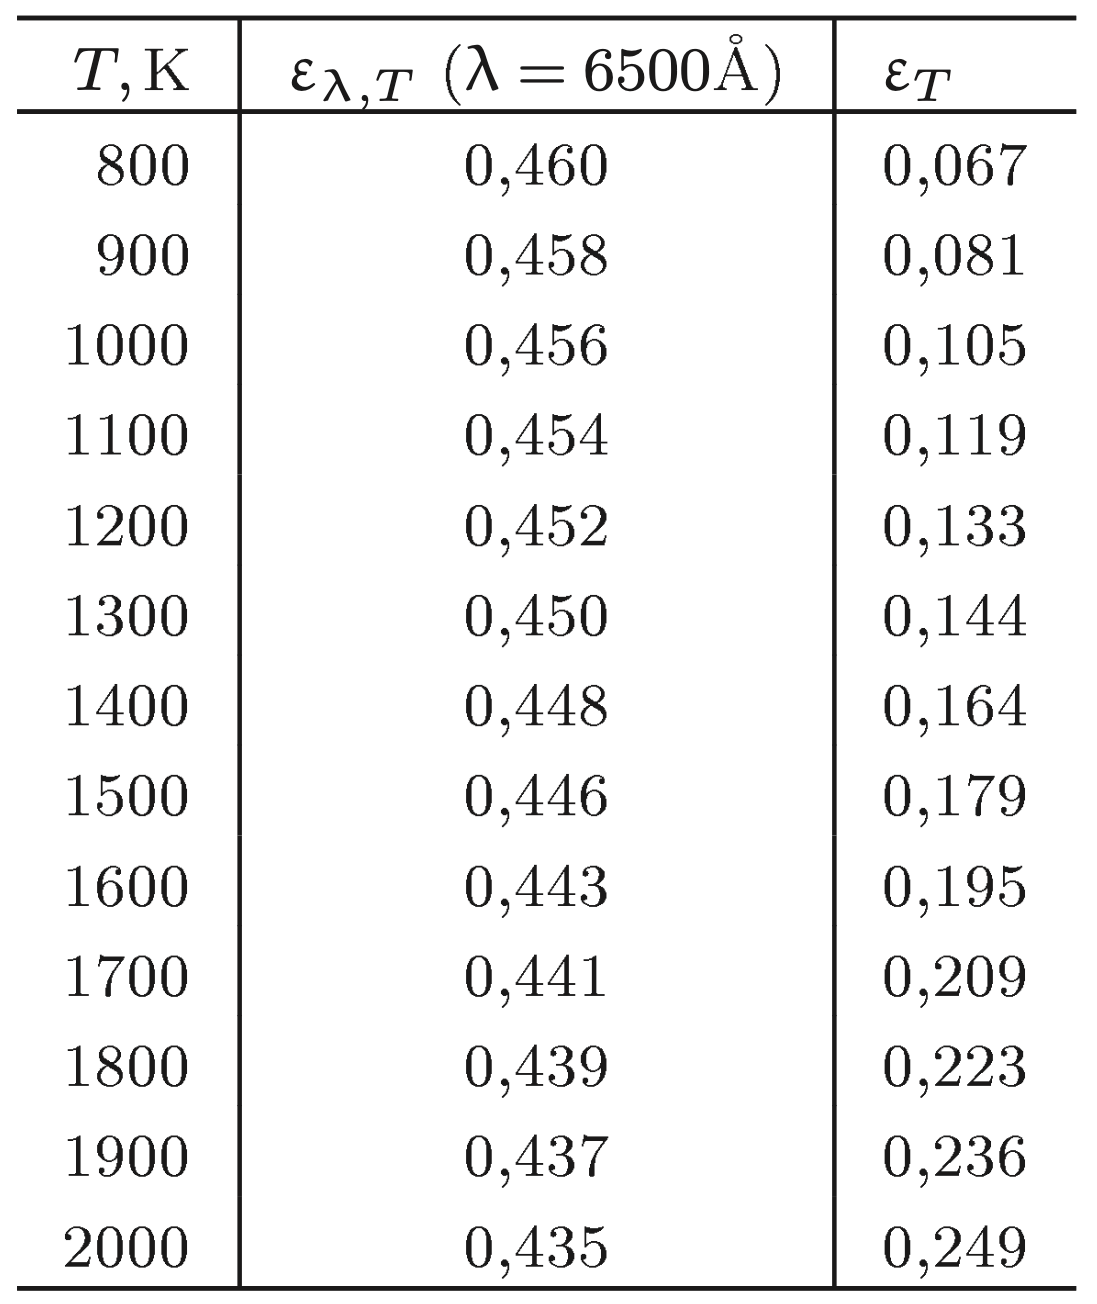
\includegraphics[width=\linewidth]{2}
    \caption{Эффект Поккельса --- появление новых главных направлений
    при наложении электрического поля}
    \label{fig:2}
\end{wrapfigure}

Измеряя радиусы колец, можно найти разность $(n_o-n_e)$ ---
двулучепреломление кристалла. Свойства симметрии кристалла и его
электрооптический тензор таковы, что в результате линейного
электрооптического эффекта в плоскости $(xy)$ возникают два главных
направления $\xi$ и $\eta$ под углами $45^\circ$ к осям $x$ и $y$
(\fig{fig:2}) с показателями преломления $(n_o-\Delta n)$ и $(n_o+
\Delta n)$, то есть появляются <<медленная>> и <<быстрая>> оси, причем
$\Delta n = A \cdot E_\text{эл}$ ($A$ --- некая константа, зависящая
только от типа кристалла).

Интенсивность света пропорциональна
квадрату модуля вектора электрического поля в волне:
\[
    I_\text{вых} \sim EE^{*} = E_0^2\sin^2 \left( \frac{\Delta \phi}{2}
        \right),
\]
поэтому 
\begin{equation}
    I_\text{вых} = I_0 \sin^2 \left( \frac{\Delta \phi}{2}\right) =
    I_0 \sin^2 \left( \frac{\pi}{2} \frac{U}{U_{\lambda/2}}\right) 
    \label{eq:3}
\end{equation}
Здесь
\begin{equation}
    U_{\lambda/2} = \frac{\lambda}{4 A} \frac{d}{l}
    \label{eq:4}
\end{equation}
--- так называемое полуволновое напряжение --- имеет тот смысл, что
при $U = U_{\lambda/2}$ сдвиг фаз между двумя волнами,
соответствующими двум собственным поляризациям, $\Delta \phi = \pi$
(разность хода равна $\lambda/2$), и интенсивность света на выходе
анализатора, как следует из \eqref{eq:3}, достигаем максимума.

При параллельных поляризациях лазера и анализатора 
\begin{equation}
    I_\text{вых} = I_0 \cos^2 \left( \frac{\pi}{2}
    \frac{U}{U_{\lambda/2}} \right)
    \label{eq:5}
\end{equation}

Напряжение $U_{\lambda/2}$ называют также управляющим напряжением. Оно
уменьшается, как видно из \eqref{eq:4}, с уменьшением длины волны
света $\lambda$ и с увеличением отношения $\lambda/d$ кристалла.
Характерная величина полуволнового напряжения в ниобате лития для
видимого света составляет несколько сотен вольт.






\section{Оборудование}
\textbf{В работе используются:} гелий-неоновый лазер, поляризатор,
кристалл ниобата лития, матовая пластинка, экран, источник
высоковольтного переменного и постоянного напряжения, фотодиод,
осциллограф, линейка.


\begin{figure}[H]
    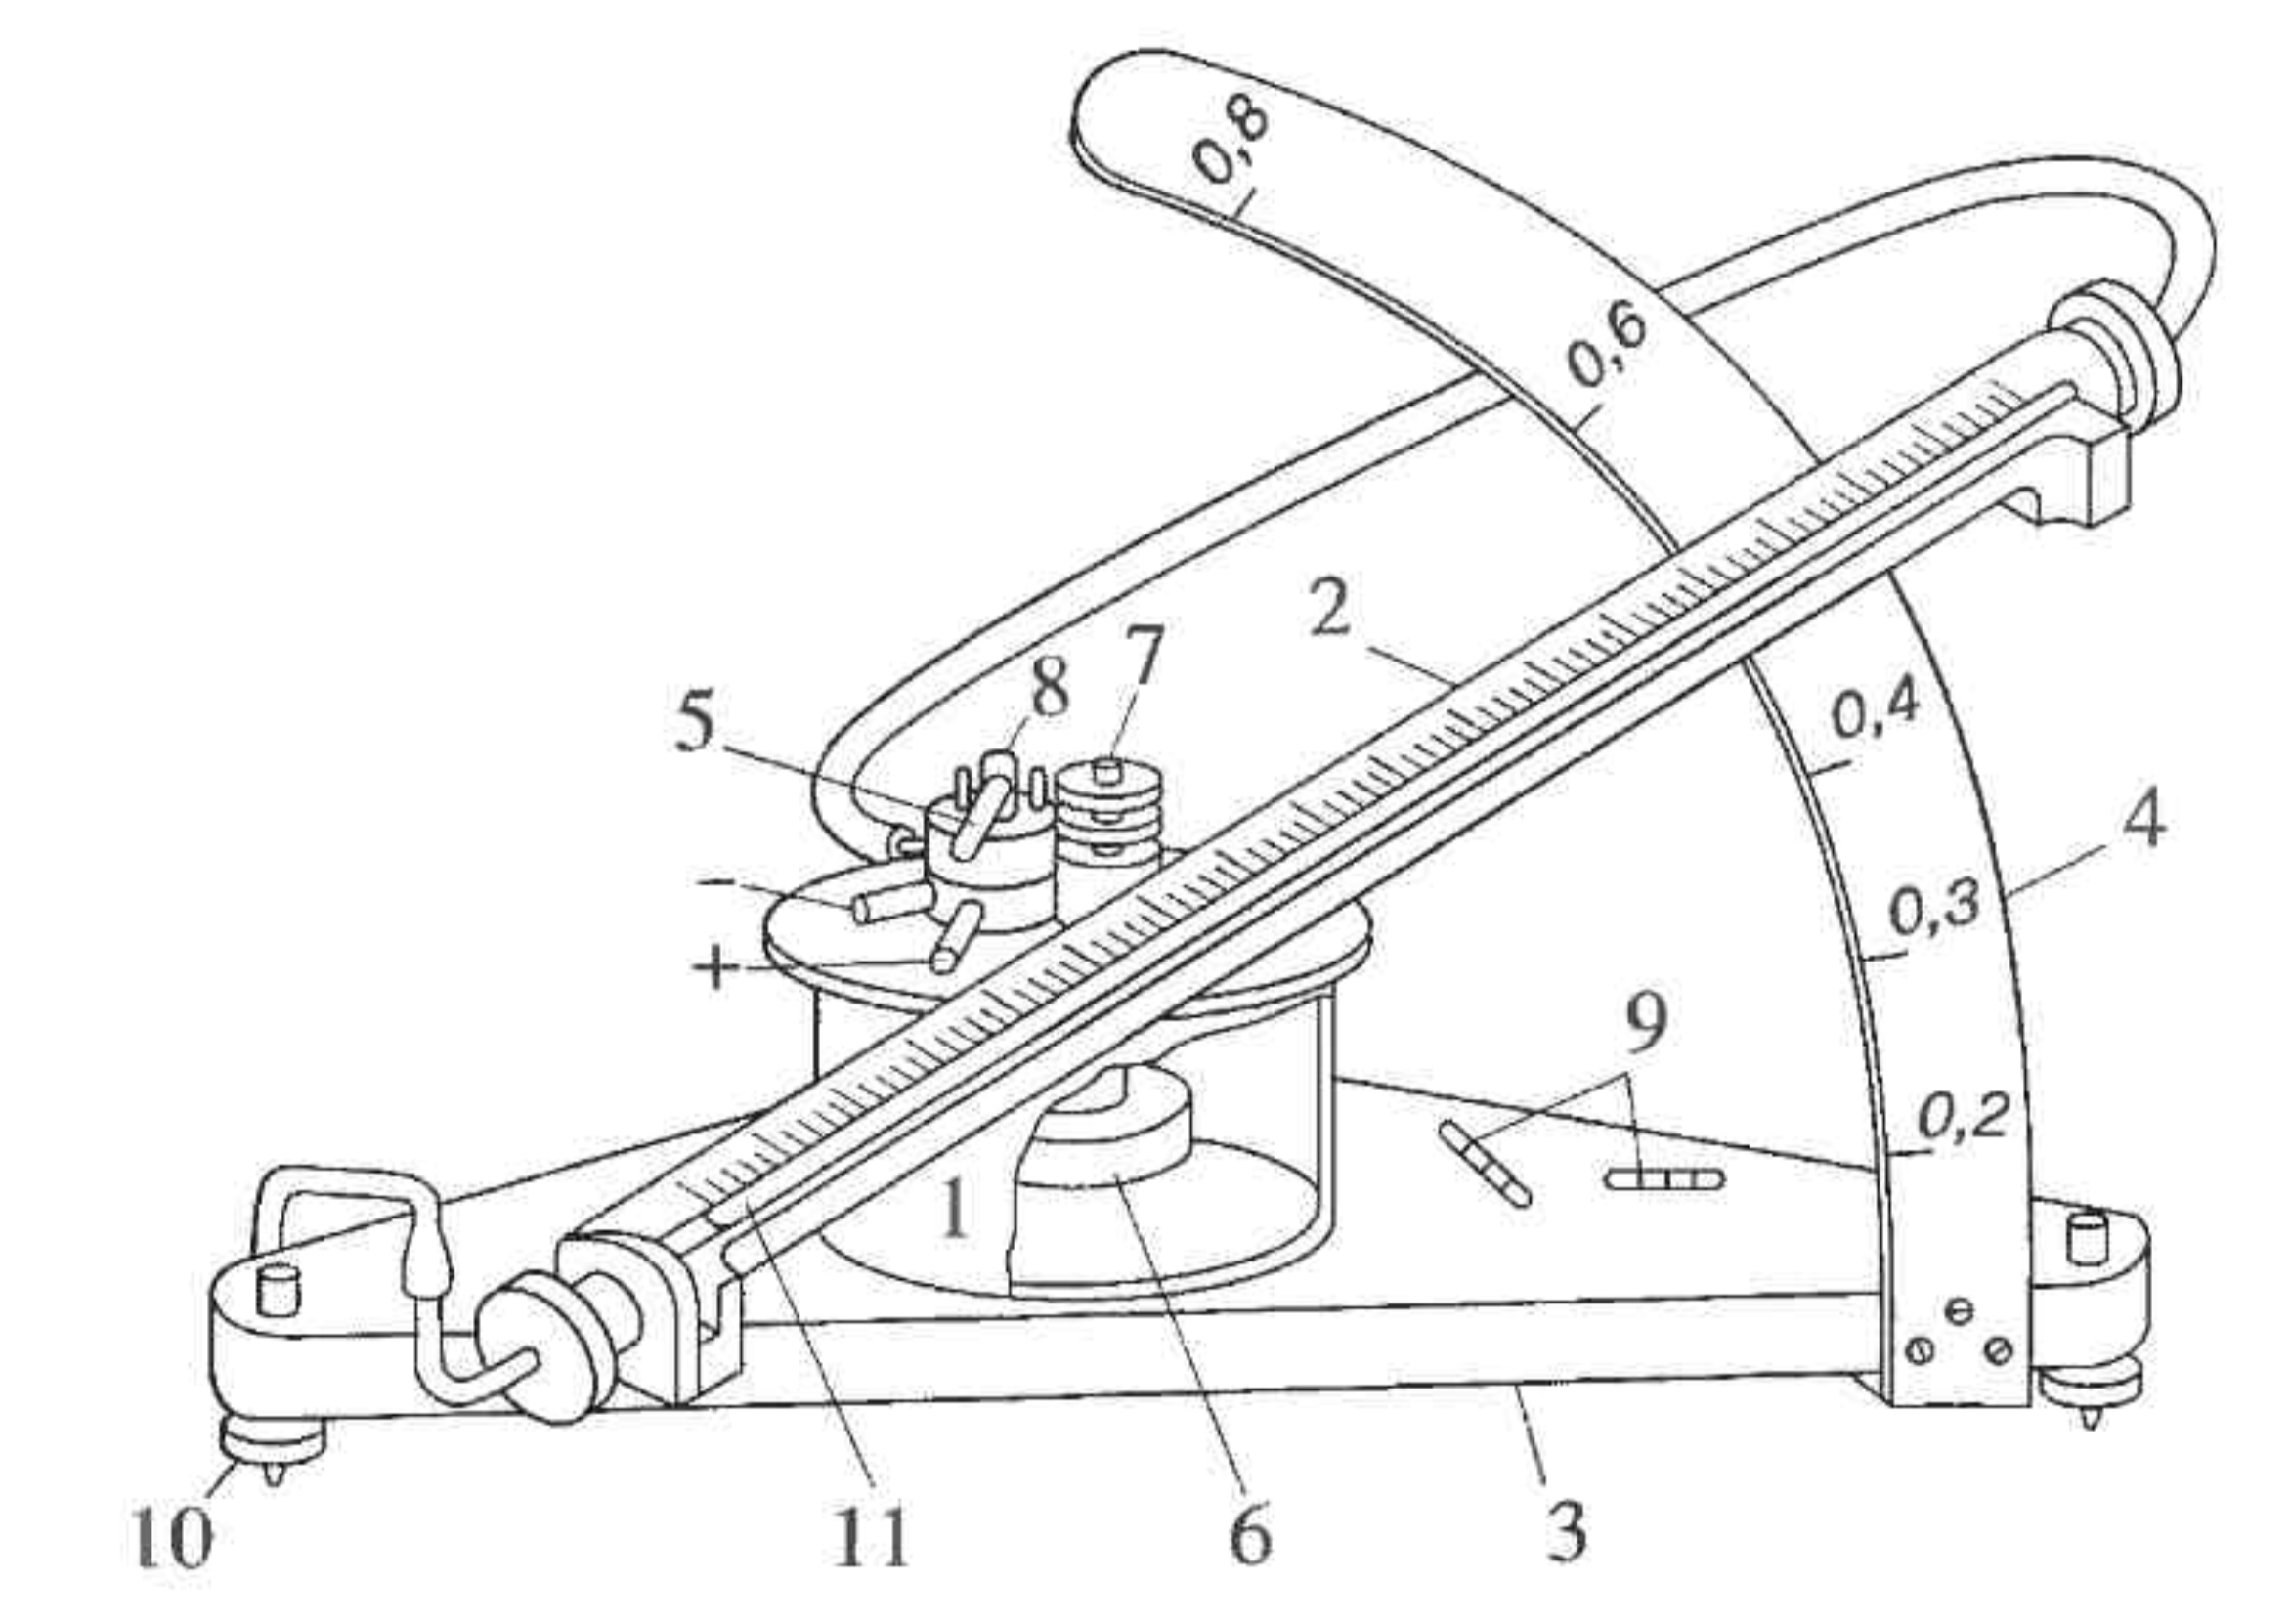
\includegraphics[width=0.8\linewidth]{3} 
    \caption{Схема для изучения двойного лучепреломления в
    электрическом поле}
    \label{fig:3}
\end{figure}

Оптическая часть установки представлена на \fig{fig:1}. Свет
гелий-неонового лазера, поляризованный в вертикальной плоскости,
проходя сквозь матовую пластинку, рассеивается и падает на
двоякопреломляющий кристалл под различными углами. На экране,
расположенном за скрещенным поляроидом, видна интерференционная
картина.

Заменив экран фотодиодом (\fig{fig:3}) и подав на кристалл перменное
напряжение, можно исследовать поляризацию луча с помощью осциллографа.



\section{Результаты измерений и обработка результатов}
Длина волны гелий-неонового лазера
\[
    \lambda = 0,63\ \text{мкм}
\]

Показатель преломления $n_o$:
\[
    n_o = 2,29
\]

Размеры кристалла:
\[
    3\times 3 \times 26\ \text{мм} \Rightarrow l = 26\ \text{мм}
\]

Измерим радиусы темных колец $r(m)$ и расстояние $L$ от середины
кристалла до экрана. 

\renewcommand{\arraystretch}{1.2}
\begin{table}[H]
\centering
\begin{tabular}{|c|c|c|c|c|c|c|c|c|}
\hline
                  & $m$ & 1  & 2  & 3  & 4  & 5  & 6  & 7  \\ \hline
    \multirow{2}{*}{$L = 915\ \text{мм}$} & $r,\ \text{мм}$ & 33 & 47 & 58 & 65 & 74 & 88 & 93 \\ \cline{2-9} 
                   & $r,\ \text{мм}$ & 30 & 43 & 55 & 65 & 72 & 88 &    \\ \hline
\multirow{2}{*}{$L = 460\ \text{мм}$} & $r,\ \text{мм}$ & 17 & 25 & 30 & 36 & 40 & 44 & 46 \\ \cline{2-9} 
                   & $r,\ \text{мм}$ & 16 & 24 & 30 & 35 & 38 & 42 & 46 \\ \hline
\end{tabular}
\caption{Радиусы темных колец $r(m)$ и расстояние $L$ от середины
кристалла до экрана}
\end{table}

Погрешности измерений равны: $\sigma_L = 10\ \text{мм}$, $\sigma_r =
5\ \text{мм}$. Основной вклад в погрешность вносит систематическая
погрешность измерения линейкой.

Построим график $r^2 = f(m)$. 
\begin{figure}[H]
    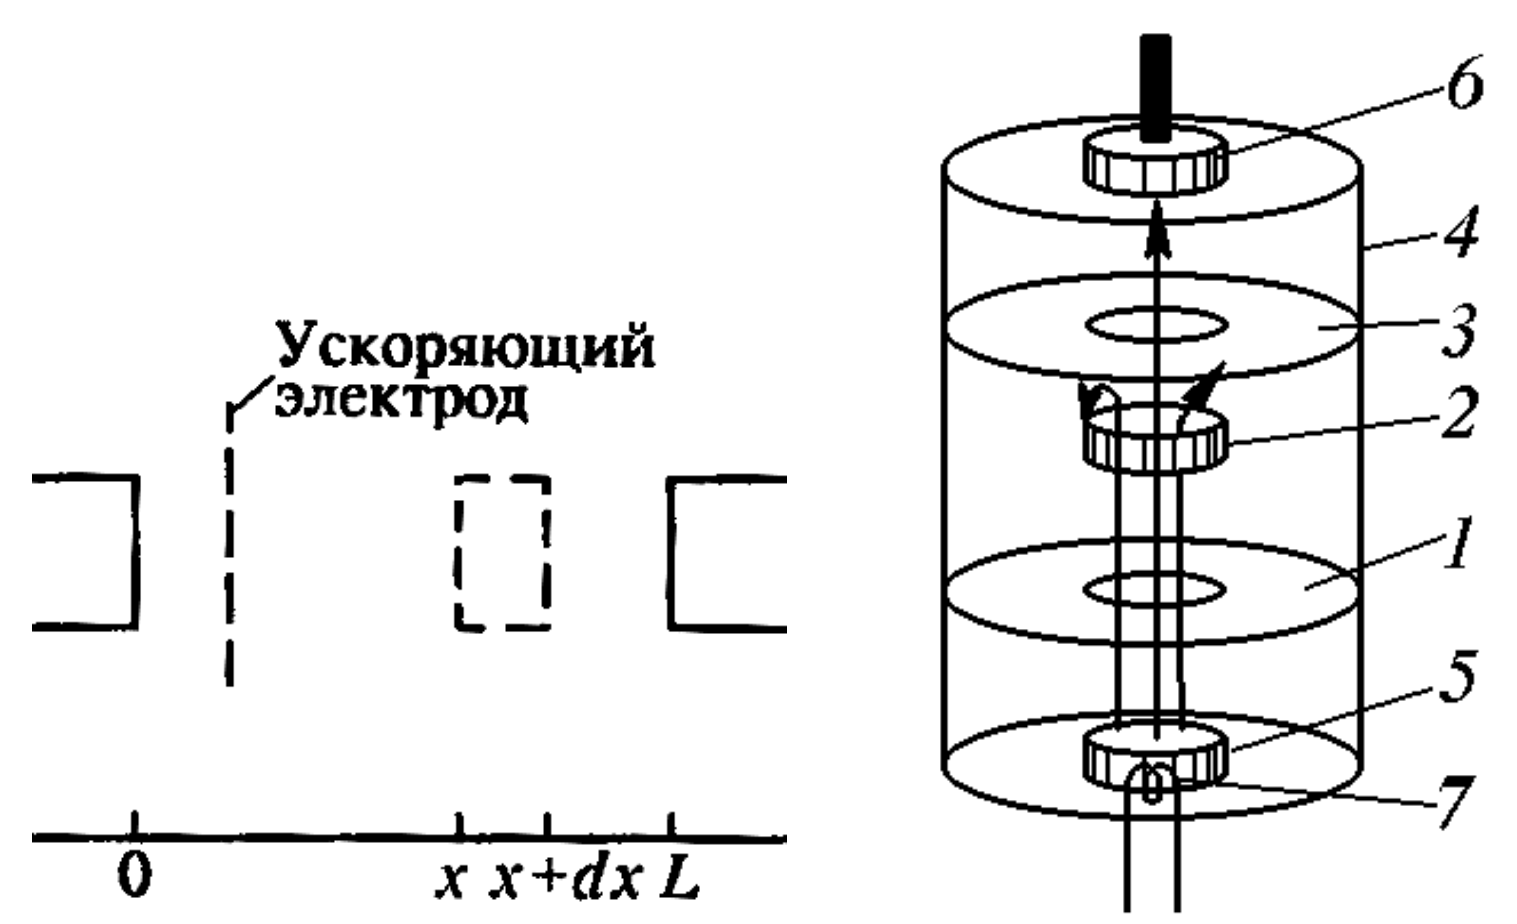
\includegraphics[width=\linewidth]{4} 
    \caption{График зависимости квадрата радиуса колец $r^2$ от номера
    темных полос $m$}
    \label{fig:4}
\end{figure}

Аппроксимация прямой графика на \fig{fig:4} подтверждает верность
формулы~\eqref{eq:2}. По углу наклона прямой определим
двулучепреломление $(n_o-n_e)$ ниобата лития, пользуясь формулой
\eqref{eq:2}:
\[
    n_o - n_e = \frac{\lambda}{k l}(n_o L)^2
\]
Усредняя по двум прямым:
\[
    n_o - n_e = 0,089\pm 0,006
\]

Для скрещенных поляризаций при напряжениях $U = (2k-1)U_{\lambda/2}$
наблюдается максимум интенсивности, при $U = 2k U_{\lambda/2}$ ---
минимум, здесь $k$ --- натуральное число. Для параллельных поляризаций
ситуация противоположная.

\begin{table}[H]
\centering
\begin{tabular}{|c|c|c|}
\hline
 & \specialcell{Скрещенные\\[-5pt]поляризации}    &
\specialcell{Параллельные\\[-5pt]поляризации} \\ \hline
$U_{\lambda/2},\ \text{В}$ & 390  & 390  \\ \hline
$U_{\lambda},\ \text{В}$ & 900  & 870  \\ \hline
$U_{3\lambda/2},\ \text{B}$ & 1440 & 1470 \\ \hline
\end{tabular}
\caption{Напряжения соответствующие последовательным экстремума
интенсивности для различных поляризаций}
\end{table}

Усредняя, получим:
\[
    U_{\lambda/2} = 439 \pm 39\ \text{В}
\]

Установим вместо экрана фотодиод (\fig{fig:3}) и подключим его $y$ -
входу осциллографа. Убрав напряжение до нуля, переключим разъем с
постоянного на переменное напряжение. С трехвольтового выхода блока
питания подаем сигнал на вход $x$ осциллографа. Отклонение луча
осциллографа по оси $x$ будет пропорционально напряжению $U$ на
кристалле, а по оси $y$ --- интенсивности прошедшего через анализатор
сигнала $I_\text{вых}$.

Постепенно повышая напряжение на кристалле, наблюдаем на экране
осциллографа фигуры Лиссажу, соответствующие зависимости
$I_\text{вых}(U)$ для скрещенных поляризаций лазера и анализатора.

Слегка поворачивая кристалл, сделаем фигуры Лиссажу симметричными.
Определим по фигурам Лиссажу полуволновое напряжение $U_{\lambda/2}$
как $\Delta U$, соответствующее переходу от максимума к минимуму
сигнала на осциллограмме:


\begin{table}[H]
\centering
\begin{tabular}{|c|c|c|}
    \hline 
    $U_{\lambda/2},\ \text{В}$ & $U_{\lambda},\ \text{В}$ &
    $U_{3\lambda/2},\ \text{В}$ \\ \hline 
    420 & 870 & 1380 \\ \hline 
\end{tabular}
\caption{Напряжение, соответствующее переходу от максимума к минимуму
сигнала на осциллограмме}
\end{table}

Определим полуволновое напряжение:
\[
    U_{\lambda/2}^{*} = 438 \pm 17\ \text{B}
\]



\section{Обсуждение результатов и выводы}
В работе изучена интерференция рассеянного света, прошедшего кристалл
ниобата лития: получена зависимость квадрата радиуса темного кольца
интерференционной картины от номера минимума $r_m^2(m)$, с хорошей
точностью являющаяся линейной (\fig{fig:4}), что
согласуется с теорией при малых углах отклонения луча от оптической
оси кристалла и близких значениях показателей преломления для
обыкновенной и необыкновенной волн. Действительно, двулучепреломление
кристалла $n_o - n_e$ составляет
\[
    n_o - n_e = 0,089\pm 0,006
\]
Это значение соответствует литиевым кристаллам. 
	
Рассмотрен эффект Поккельса: несколькими способами определено
полуволновое напряжение, оно совпадает в пределах погрешности
и равно
\begin{equation}
    \begin{gathered}
        U_{\lambda/2} = 439 \pm 39\ \text{В} \\
        U_{\lambda/2}^{*} = 438 \pm 17\ \text{В}
    \end{gathered}
\end{equation}

Получены фигуры
Лиссажу, отражающие зависимость интенсивности выходного
сигнала от подаваемой амплитуды напряжения $I(U)$ при
скрещенных и параллельных поляризациях. Картинки для
поляризаций отличаются по фазе на $\pi/2$.



\end{document}
